% Adapted from PHGST-DM_article_source/main.tex, original Section 5.
\chapter{Experiments and Analysis}
\label{ch:experiments}
\label{sec:exp}

The Process-Informed Heterogeneous-Graph Spatiotemporal Transformer with Delay-aware Modeling (PHGST-DM) jointly predicts the bottleneck station, onset, duration, observable process cause, and remaining order time. Its inputs combine resource observations on a heterogeneous process--logistics graph with recurrent temporal-pattern context.

We evaluate whether PHGST-DM can address limitations in observation scope and bottleneck supervision when forecasting bottleneck events, process causes, and remaining order time. Baseline comparisons evaluate these joint outputs; component studies examine heterogeneous multi-entity representation, process-informed supervision and temporal pattern clustering, and recurrent-pattern-guided delay-aware modelling. A case study follows bottleneck onset, persistence, and recovery. Together, these evaluations assess how the proposed designs contribute to advance warning and joint forecasting. Supplementary results and attention analyses are reported in Appendices~\ref{app:supplementary-results} and~\ref{app:attention-analysis}.

\FloatBarrier
\section{Experimental setup}

\subsection{Dataset and data processing}

Experiments use \texttt{dense\_i1}, collected from an open-workspace factory model developed in NVIDIA Isaac Sim. This dataset identifier denotes the collection with one active operating-variation dimension at intensity level 1, together with nominal episodes. Each episode produces ten workpieces through cutting, grooving, spot welding, root welding, surface welding, and finishing (Figure~\ref{fig:experiment}). The graph contains 38 nodes: seven workstations, four gantries, five workers, four transport robots (AGVs), and 18 buffers. The seven workstations, four gantries, and four AGVs are the 15 prediction targets; worker, buffer, and resource-associated material features supply context. Each resource is represented by 27 features, and observations are aggregated into one-minute windows.

\begin{figure}[!htbp]
\centering
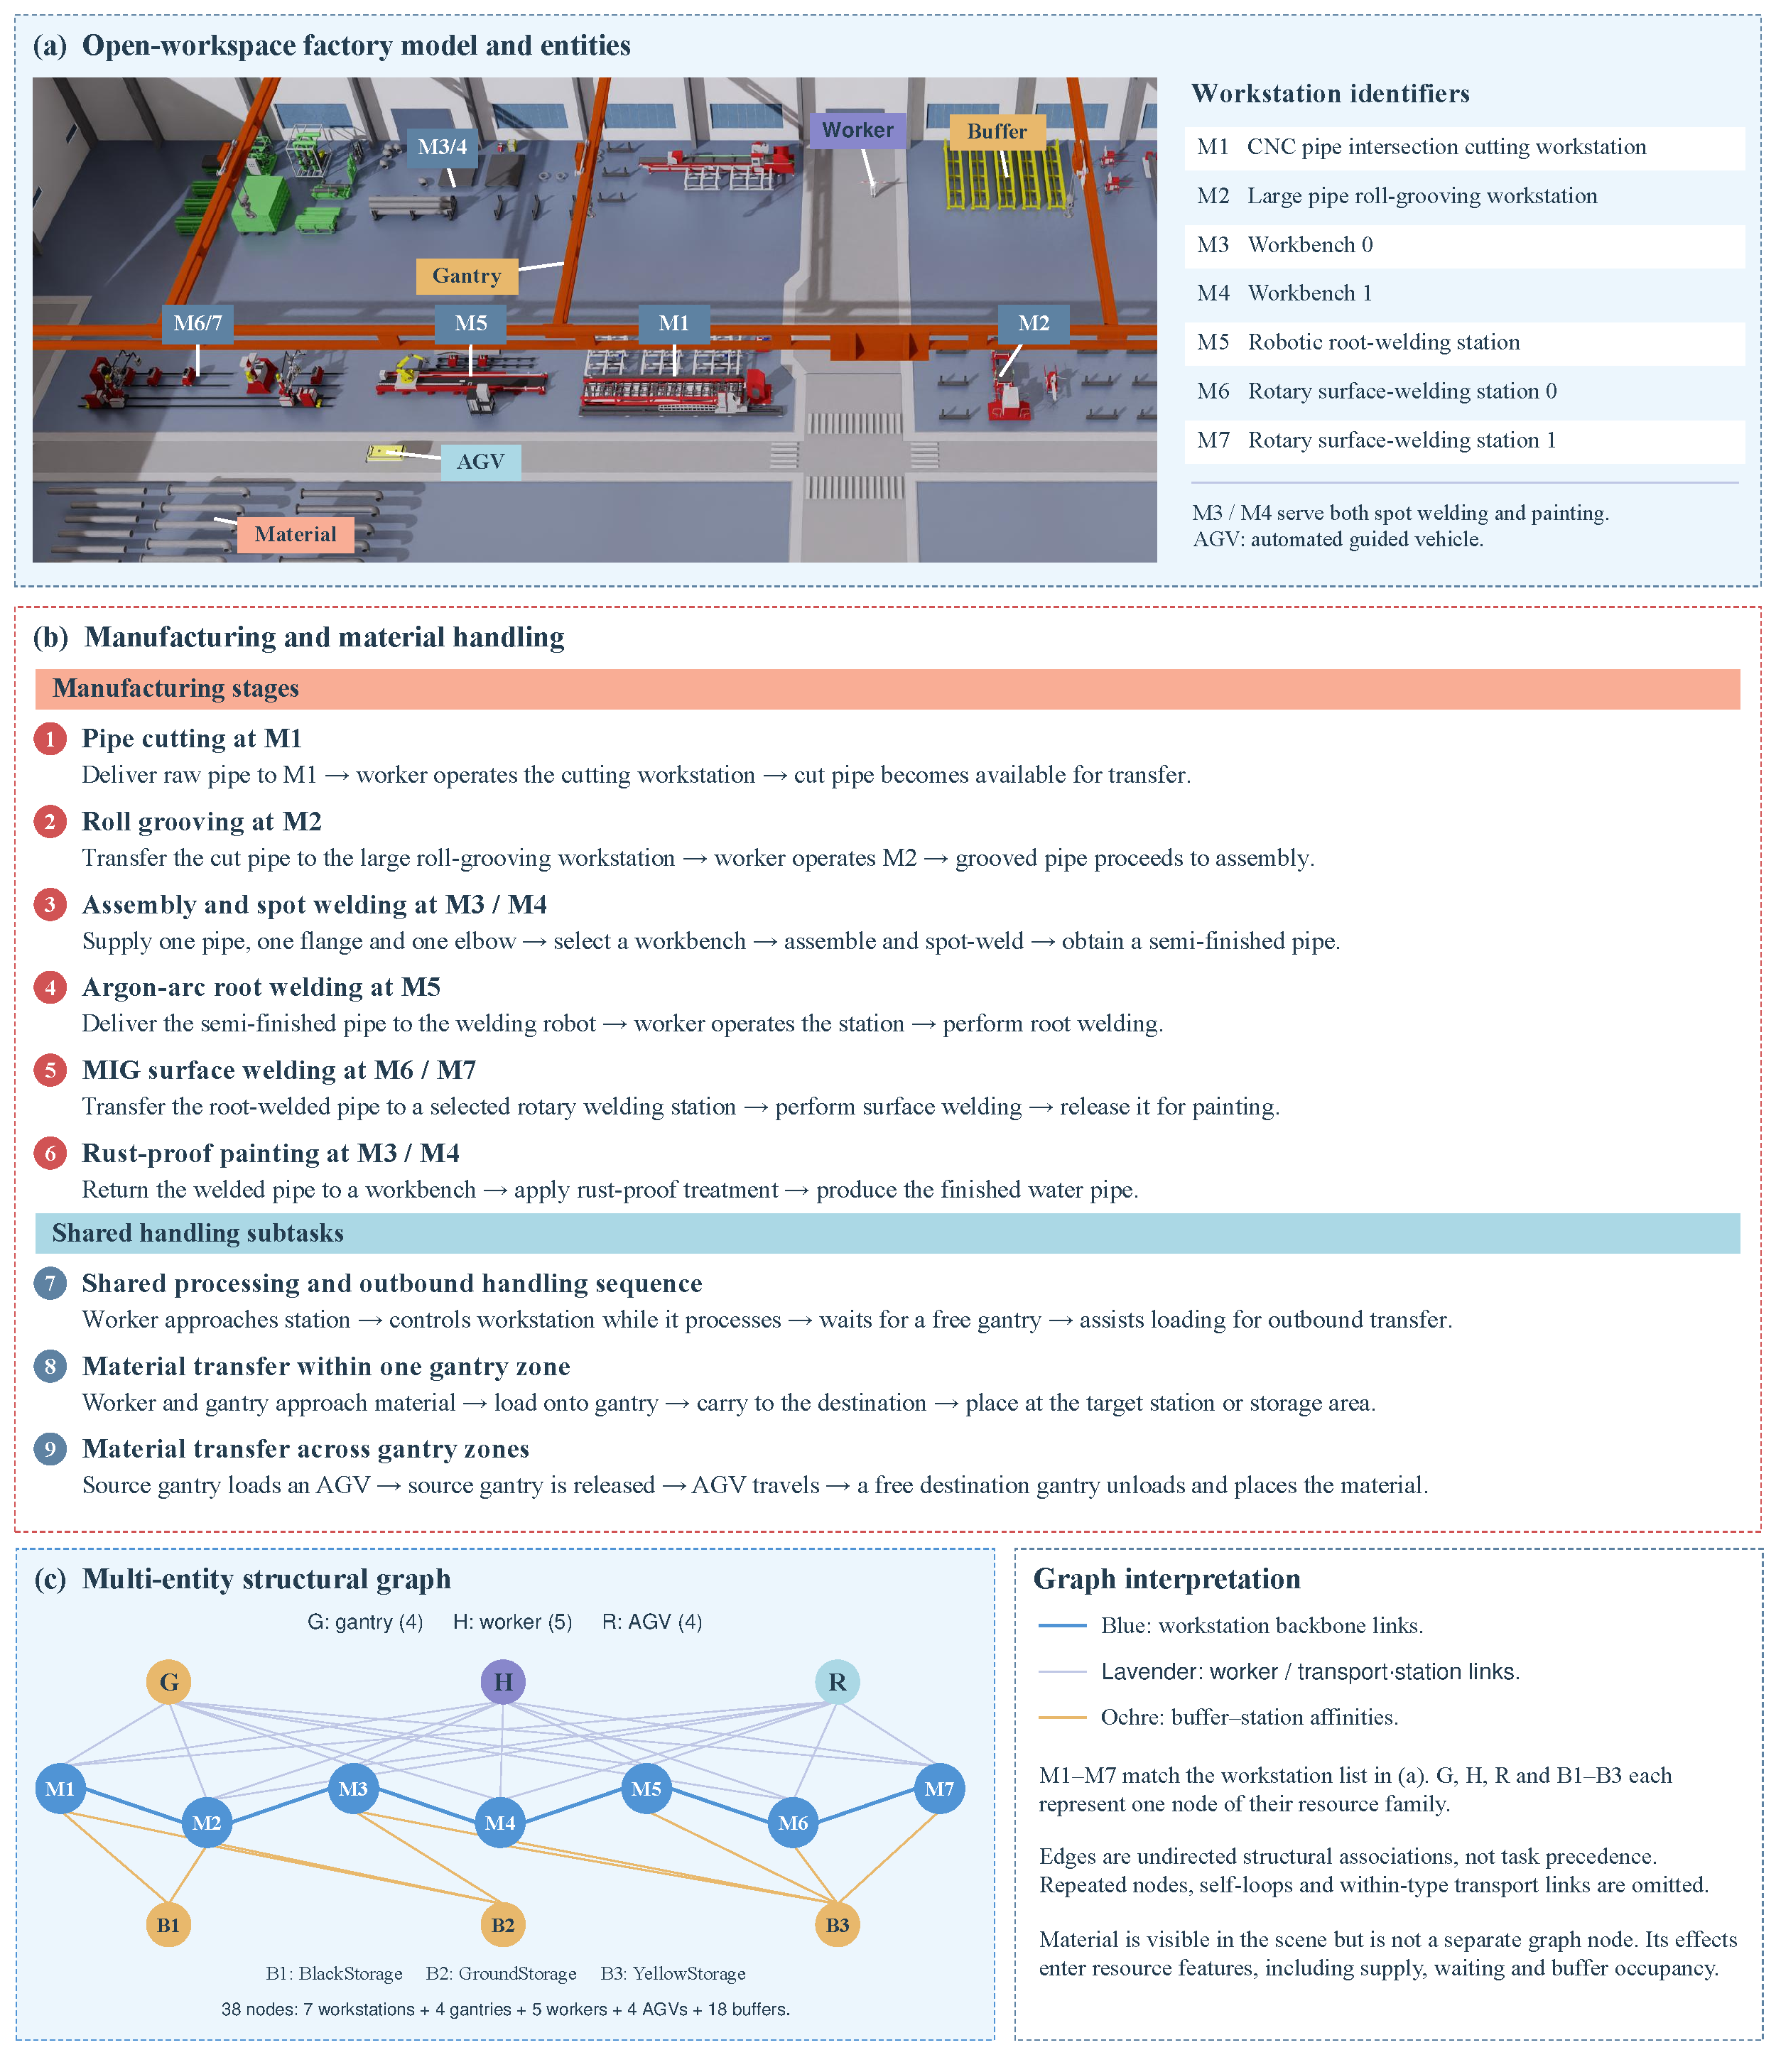
\includegraphics[width=\linewidth]{figures/fig_experiment.pdf}
\caption{Open-workspace factory model developed for NVIDIA Isaac Sim: (a)~resource entities; (b)~manufacturing stages; (c)~structural graph of 38 resources.}
\label{fig:experiment}
\end{figure}

The data-generation environment exposes four operating variation dimensions and applies variations in each dimension at three intervention levels (Table~\ref{tab:disturbance-design}). Level~0 changes episode-wide resource capacity before each model run, Level~1 perturbs sampled processing or service behaviour, and Level~2 injects temporary events during production. The platform supports intensity $I\in\{1,2,3\}$; slash-separated values in the table follow this order. The main \texttt{dense\_i1} collection activates one dimension at a time at $I=1$, while nominal runs keep all dimensions inactive. The injected dimension controls data generation but is not used as the bottleneck or process-cause label.

\begin{table}[!htbp]
\centering
\caption{Four operating variation dimensions and their three intervention levels. Values separated by slashes correspond to $I=1/2/3$. One model step equals one logical second.}
\label{tab:disturbance-design}
\footnotesize
\setlength{\tabcolsep}{3.2pt}
\renewcommand{\arraystretch}{1.12}
\begin{tabularx}{\linewidth}{@{}p{0.13\linewidth}YYY@{}}
\toprule
Dimension & L0: episode configuration & L1: sampled process variation & L2: temporary runtime events \\
\midrule
Workstation & Disable workbench ws1 and rotary-welding ws1 & Processing-time noise $5/10/15$ steps; success rate $0.88/0.76/0.64$; tool wear $15/30/45$ steps per 1,000 steps & $2/(2$--$3)/(3$--$4)$ idle-station failures; additional $1$--$2/2$--$3/3$--$4$ weld or kitting quality-hold windows \\
Worker & Reduce the number of workers from 5 to $3/2/1$ & Service-time scale $1.55/2.10/2.65$; worker-specific skill range $0.8$--$1.4/0.7$--$1.6/0.6$--$1.8$; time noise $12/22/32$ steps & $2/(2$--$3)/(3$--$4)$ temporary absences, applied only when the selected worker is idle \\
Logistics & Reduce the number of AGVs from 4 to $2/1/1$; retain all four zone gantries & Gantry-time scale $1.65/2.30/2.95$ with motion noise $10/18/26$ steps; weak background process variation & $2/(2$--$3)/(3$--$4)$ gantry or AGV freezes; at least one pulse targets an AGV while other vehicles remain active \\
Material & Keep the nominal inventory of ten pipes, flanges, and elbows; no permanent deletion & At steps 400--1,000, temporarily hide $6$--$7/7$--$8/7$--$8$ idle flanges or elbows for $1{,}400$--$2{,}200/2{,}000$--$2{,}700/2{,}500$--$3{,}200$ steps & After the opening shortage, inject $1$--$2/2$--$3/3$--$4$ complementary flange/elbow shortage pulses; pipe blanks are never hidden \\
\bottomrule
\end{tabularx}
\end{table}

For workstation, worker, and logistics operating variations, every Level~2 pulse lasts at least 600 steps and the intensity-specific upper bounds are 900/1,300/1,400 steps. Event targets, start times, counts, and durations are resampled for each episode using a deterministic seed. Adjacent pulses are separated by at least 360 steps, and an event is delayed until an eligible target is idle rather than interrupting an active operation. These controls produce sustained operating variations while avoiding a deterministic one-to-one mapping between an injection and a labelled bottleneck.

A run-stratified, episode-level split gives 140/28/36 training/validation/test episodes from 204 valid episodes, yielding 20,826/4,331/5,354 forecast windows (Table~\ref{tab:exp-dataset}). Preprocessing uses synchronized episode logs; normalization and temporal-pattern prototypes are fitted on the training split only. Invalid episodes affected by the known simulator deadlock are excluded. All comparisons use the same test-window identities, history length, future grid, target resources, and label definitions. Table~\ref{tab:dataset-labels} reports test-label composition. All single-device trajectory comparisons and the case study use the same cutting workstation (\texttt{num02}) from the same test episode; the selection procedure is documented in Appendix~\ref{app:case-details}.

Process-informed labels combine resource-specific operational evidence, filter short runs, and fill one-window internal gaps. At inference, the model uses the observed history rather than retrospective future occupancy. The onset limit is the maximum admissible offset of a newly emerging bottleneck; experiments compare limits of 5, 10, and 15~min. Bottleneck events are required to persist for at least 8~min ($m=8$ one-minute windows), with ongoing events evaluated over their remaining duration. The future label grid remains fixed at 30 windows. Strict report matching uses a three-window onset tolerance; timing errors are reported in minutes. In the label summary below, Upcoming denotes a newly emerging event, Ongoing denotes an event already active at the forecast origin, and No-event denotes a pair with no eligible event.

\begin{table}[!htbp]
\centering
\caption{Dataset and label protocol used in the experiments.}
\label{tab:exp-dataset}
\footnotesize
\setlength{\tabcolsep}{4pt}
\renewcommand{\arraystretch}{1.08}
\begin{tabularx}{\linewidth}{@{}>{\raggedright\arraybackslash}p{\dimexpr 0.30\linewidth + 1cm\relax}@{\hspace{0.03\linewidth}}>{\raggedright\arraybackslash}X@{}}
\toprule
Item & Setting \\
\midrule
Dataset & \texttt{dense\_i1}, 204 valid episodes, 38 resources \\
Split & 140/28/36 episodes; 20,826/4,331/5,354 windows \\
Windowing & 60-s windows; 30 historical + 30 future windows \\
Targets & 15 resources: 7 workstations, 4 gantries, 4 robots \\
Onset limit & $5/10/15$~min \\
Report matching & Three-window onset tolerance \\
\bottomrule
\end{tabularx}
\end{table}

\begin{table}[!htbp]
\centering
\caption{Test-set label composition by onset limit. Counts are window--resource pairs over 5,354 windows $\times$ 15 targets; percentages are shares of all pairs.}
\label{tab:dataset-labels}
\footnotesize
\setlength{\tabcolsep}{3.2pt}
\renewcommand{\arraystretch}{1.08}
\begin{tabularx}{\linewidth}{@{}>{\raggedright\arraybackslash}p{0.24\linewidth}>{\raggedleft\arraybackslash}X>{\raggedleft\arraybackslash}X>{\raggedleft\arraybackslash}X@{}}
\toprule
Onset limit & Upcoming & Ongoing & No-event \\
\midrule
$\leq5$ & 336 (0.42\%) & 766 (0.95\%) & 79,208 (98.63\%) \\
$\leq10$ & 604 (0.75\%) & 768 (0.96\%) & 78,938 (98.29\%) \\
$\leq15$ & 708 (0.88\%) & 770 (0.96\%) & 78,832 (98.16\%) \\
\bottomrule
\end{tabularx}
\end{table}

\subsection{Baseline methods}

Four baselines represent recurrent, graph-based, and Transformer forecasting approaches. LSTM models historical sequences; BSTAN combines graph attention with GRU for blockage/starvation-related prediction~\citep{lai2023bstan}; BTGCN combines production-task graphs with GCN and GRU~\citep{yin2025btgcn}; and PDFormer is adapted from its propagation-delay-aware Transformer architecture for bottleneck prediction~\citep{jiang2023pdformer}. All baselines follow the unified experimental protocol, with architecture-specific input representations and learning algorithms. The validation-only fallback rule is documented in Appendix~\ref{app:additional}.

\begin{table}[!htbp]
\centering
\caption{Baseline models and their roles in the comparison.}
\label{tab:exp-baselines}
\footnotesize
\setlength{\tabcolsep}{4pt}
\renewcommand{\arraystretch}{1.10}
\begin{tabularx}{\columnwidth}{@{}lXX@{}}
\toprule
Model & Core framework & Comparison role \\
\midrule
LSTM & Long short-term memory & Recurrent temporal predictor \\
BSTAN & Graph attention + GRU & Graph-attention predictor \\
BTGCN & Graph convolution + GRU & Graph-convolutional predictor \\
PDFormer & Propagation-delay-aware Transformer & Spatiotemporal Transformer predictor \\
\bottomrule
\end{tabularx}
\end{table}

\subsection{Overall experimental settings and metrics}

All experiments use common data splits, forecast windows, targets, initialization controls, training-budget standards, and validation-based selection. Full and ablation models start from the same fixed parameter state; all selected models and report thresholds are frozen before testing.

Shared PHGST-DM settings appear in Table~\ref{tab:shared-training-protocol}. Training uses AdamW with a batch size of 16, a learning rate of $5\times10^{-5}$, a weight decay of $0.05$, cosine learning-rate decay to $10^{-6}$, and fourfold positive-window oversampling. Under the two-stage training procedure, stage~1 starts from the fixed parameter state shared by all ablation arms, unfreezes all five encoder blocks, and runs for at most 50 epochs with an early-stopping patience of 40. Far-onset weighting doubles onset loss beyond 5~min and uses positive weights $9/10/11$ for the three limits; ordinary and hard false-positive weights are $2.5$ and $2.2$. Stage~2 runs for at most 20 epochs, with the checkpoint selected by validation loss. All runs use seed 42 and provide point estimates rather than multi-seed stability estimates. Appendix~\ref{app:additional} provides loss weights, label thresholds, and decoding details.

The model and report threshold are selected on the validation split. Candidate thresholds are listed explicitly in Table~\ref{tab:shared-training-protocol}; selection uses the internal station-identification F1 among candidates satisfying validation report precision $\geq0.80$ and recall $\geq0.70$. This selection score is not reported as a result; the reported event metric is the onset-qualified F1-score defined below. PHGST-DM uses the selected threshold of $0.94$ for testing at all three onset limits.

For resource $n$ at forecast origin $t$, let $\hat s_{t,n}$ and $s_{t,n}$ denote the predicted and reference onset offsets in minutes. A strict report-level hit requires the correct resource and an absolute onset error within tolerance $\epsilon_s$:
\begin{equation}
|\hat{s}_{t,n}-s_{t,n}|\leq\epsilon_s,\qquad
\epsilon_s=3~\mathrm{min}.
\end{equation}
At the one-minute window resolution, this tolerance equals three windows.

Metrics cover bottleneck-event prediction, process-cause classification, and remaining order time. The reported bottleneck-event F1-score requires both correct station identification and an onset error within three windows. Upcoming recall uses future-event window--resource pairs whose final historical window is non-bottleneck; Ongoing recall uses pairs with an active final historical window. Mean absolute error (MAE) for onset and duration is measured on correctly detected events, while union duration MAE and root mean squared error (RMSE) include missed events and false positives. Event F1 is the harmonic mean of precision and recall; macro recall is the unweighted mean of class-specific recalls. Next-window and 30-window State F1 describe the predicted occupancy over time, including recovery. Process-cause evaluation uses accuracy and macro recall over the four supported classes. Order-completion evaluation uses remaining-time MAE at the line level.

\begin{table}[!htbp]
\centering
\caption{Metrics used in the main evaluation and component analyses.}
\label{tab:exp-metrics}
\footnotesize
\setlength{\tabcolsep}{3.5pt}
\renewcommand{\arraystretch}{1.08}
\begin{tabularx}{\linewidth}{@{}p{0.14\linewidth}p{0.27\linewidth}Y@{}}
\toprule
Group & Metric & Interpretation \\
\midrule
Event & F1-score & Correct station and onset within three windows \\
Warning & Upcoming / ongoing recall & Historically cold / already active resource \\
State & F1 (1 step / horizon) & Occupancy at the next window / across 30 windows \\
Temporal & Onset / duration MAE & Error on correctly detected events \\
Temporal & Union duration MAE/RMSE & Includes missed events and false positives \\
Auxiliary & Remaining-time MAE & Global order-progress error \\
Auxiliary & Cause accuracy / macro recall & Four supported process-cause classes \\
\bottomrule
\end{tabularx}
\end{table}

\FloatBarrier
\section{Overall bottleneck prediction performance}\label{sec:comparison-overview}

This section evaluates how well PHGST-DM jointly predicts bottleneck events, process causes, and remaining order time. Its performance is compared with four baselines under the shared experimental protocol (Tables~\ref{tab:comparison-main}--\ref{tab:comparison-remain}).

\subsection{Bottleneck station, onset, and duration}\label{sec:comparison-event}

At the event level, we assess how accurately PHGST-DM identifies bottleneck stations and predicts their onset, duration, and future occupancy (Table~\ref{tab:comparison-main}).

PHGST-DM achieves the highest event F1, upcoming recall, ongoing recall, and state F1 across the onset limits. Relative to the strongest baseline for each metric and limit, event F1 improves by 8.2--22.1 percentage points and upcoming recall by 28.7--39.9 percentage points. These gains show improved detection before bottlenecks become active, alongside continued coverage of persistent constraints (Figure~\ref{fig:baseline-comparison}).

\begin{table}[!htbp]
\centering
\caption{Bottleneck event and temporal prediction. Scores are percentages except timing MAE (min); best and second-best values are bold and underlined, respectively.}
\label{tab:comparison-main}
\footnotesize
\setlength{\tabcolsep}{3.2pt}
\renewcommand{\arraystretch}{1.12}
\begin{fittable}
\begin{tabular*}{\linewidth}{@{\extracolsep{\fill}}lrrrrrrr@{}}
\toprule
Model & \multicolumn{1}{c}{Event F1 $\uparrow$} & \multicolumn{2}{c}{Event recall $\uparrow$} & \multicolumn{2}{c}{Timing MAE $\downarrow$} & \multicolumn{2}{c}{State F1 $\uparrow$} \\
\cmidrule(lr){2-2}\cmidrule(lr){3-4}\cmidrule(lr){5-6}\cmidrule(l){7-8}
 & F1-score & Upcoming & Ongoing & Onset & Duration & 1 step & 30 steps \\
\midrule
\multicolumn{8}{l}{\textit{Onset limit $\leq5$}} \\
PHGST-DM & \textbf{80.4\%} & \textbf{54.2\%} & \textbf{93.7\%} & 0.127 & \textbf{1.863} & \textbf{88.3\%} & \textbf{52.5\%} \\
LSTM & 58.3\% & 9.9\% & 68.7\% & 0.056 & 3.855 & 29.5\% & 29.5\% \\
BSTAN & 68.7\% & 9.5\% & 79.4\% & 0.043 & 3.565 & 71.9\% & \underline{37.9\%} \\
BTGCN & 66.9\% & 4.6\% & 78.6\% & \underline{0.020} & 3.322 & 64.3\% & 37.2\% \\
PDFormer & \underline{72.2\%} & \underline{14.3\%} & \underline{89.2\%} & \textbf{0.008} & \underline{2.725} & \underline{85.4\%} & 34.7\% \\
\midrule
\multicolumn{8}{l}{\textit{Onset limit $\leq10$}} \\
PHGST-DM & \textbf{77.8\%} & \textbf{53.5\%} & \textbf{93.9\%} & 0.227 & \textbf{1.788} & \textbf{89.2\%} & \textbf{58.9\%} \\
LSTM & 47.7\% & 11.2\% & 69.3\% & 0.388 & 3.768 & 27.5\% & 26.2\% \\
BSTAN & \underline{60.9\%} & 5.7\% & 79.6\% & \underline{0.153} & 3.533 & 63.2\% & \underline{36.5\%} \\
BTGCN & 57.9\% & 4.5\% & 72.2\% & \textbf{0.117} & 3.238 & 56.6\% & 35.9\% \\
PDFormer & 59.8\% & \underline{22.2\%} & \underline{90.2\%} & 0.203 & \underline{2.798} & \underline{84.2\%} & 34.7\% \\
\midrule
\multicolumn{8}{l}{\textit{Onset limit $\leq15$}} \\
PHGST-DM & \textbf{76.8\%} & \textbf{53.7\%} & \textbf{93.0\%} & \underline{0.227} & \textbf{1.716} & \textbf{90.0\%} & \textbf{61.0\%} \\
LSTM & 46.1\% & 10.2\% & 64.3\% & 0.453 & 3.615 & 26.8\% & 26.0\% \\
BSTAN & 53.4\% & 4.4\% & 70.0\% & \textbf{0.222} & 3.422 & 59.3\% & 33.5\% \\
BTGCN & 51.8\% & 5.4\% & 69.9\% & 0.302 & 3.121 & 46.1\% & 32.3\% \\
PDFormer & \underline{54.7\%} & \underline{25.0\%} & \underline{89.5\%} & 0.499 & \underline{2.744} & \underline{82.2\%} & \underline{36.0\%} \\
\bottomrule
\end{tabular*}
\end{fittable}
\end{table}

Detected-event duration MAE is 0.86--1.03~min lower than that of the best baseline at each onset limit, a relative reduction of 31.6--37.5\%. This extends the benefit from identifying an affected station to estimating how long its constraint persists. Timing MAE is conditional on correct detection, and onset MAE alone does not show a uniform advantage over the baselines. Further onset-distance and resource-type results appear in Appendix~\ref{app:supplementary-results}.

\begin{figure}[!htbp]
\centering
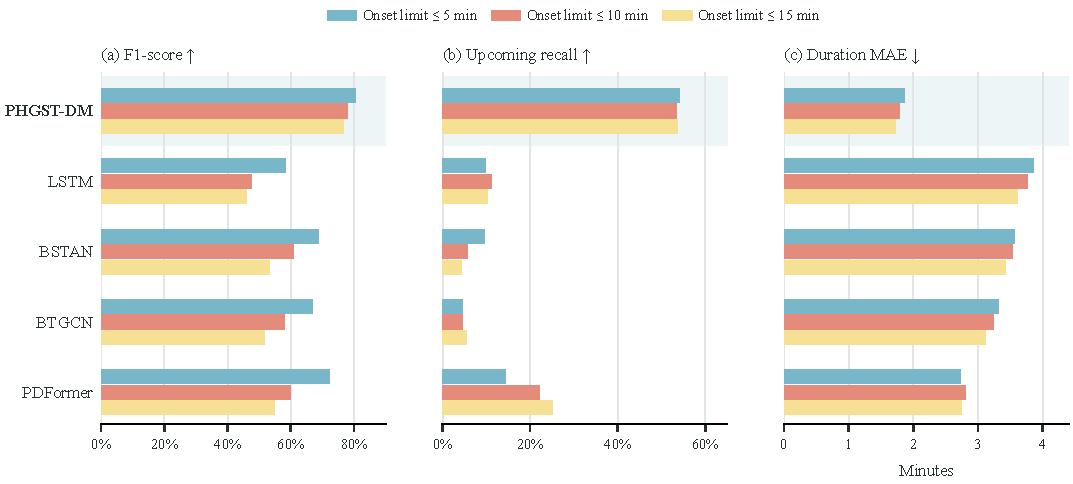
\includegraphics[width=0.96\textwidth,height=0.66\textheight,keepaspectratio]{figures/fig_range_response.pdf}
\caption{Grouped comparison of (a)~F1-score, (b)~Upcoming recall, and (c)~detected-event duration MAE across onset limits.}
\label{fig:baseline-comparison}
\end{figure}

\begin{figure}[!htbp]
\centering
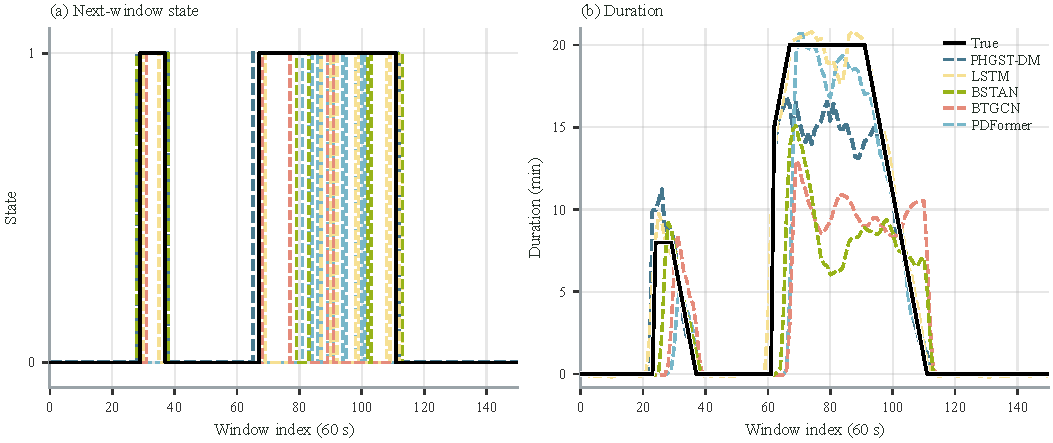
\includegraphics[width=0.90\textwidth,height=0.66\textheight,keepaspectratio]{figures/key_device_models_aligned.pdf}
\caption{Comparison of PHGST-DM and baselines at Onset limit~$\leq5$: (a)~next-window state; (b)~duration with the true reference truncated at 20~min for visualization (black: ground truth; dashed: predictions).}
\label{fig:key-device-baselines}
\end{figure}

Figure~\ref{fig:key-device-baselines} shows the corresponding trajectories. PHGST-DM tracks both bottleneck intervals and the subsequent recovery, connecting event coverage to successive duration forecasts. The displayed true-duration reference is truncated at 20~min, while every model retains the 30-min prediction horizon.

\subsection{Bottleneck process-cause prediction}\label{sec:comparison-cause}

The process-cause comparison covers four operational conditions: material shortage, transport delay, queue buildup, and downstream blockage (Table~\ref{tab:comparison-state}).

PHGST-DM outperforms the four baselines in both cause accuracy and macro recall across the onset limits. Compared with the strongest baseline at each limit, macro recall improves by 1.4--4.3 percentage points.

\begin{table}[!htbp]
\centering
\caption{Bottleneck process-cause prediction (\%). Best and second-best values are bold and underlined, respectively.}
\label{tab:comparison-state}
\footnotesize
\setlength{\tabcolsep}{3.2pt}
\renewcommand{\arraystretch}{1.12}
\begin{fittable}
\begin{tabular*}{\linewidth}{@{\extracolsep{\fill}}lrrrrrr@{}}
\toprule
Model & \multicolumn{2}{c}{Onset limit $\leq5$} & \multicolumn{2}{c}{Onset limit $\leq10$} & \multicolumn{2}{c}{Onset limit $\leq15$} \\
\cmidrule(lr){2-3}\cmidrule(lr){4-5}\cmidrule(l){6-7}
 & Accuracy $\uparrow$ & Macro R $\uparrow$ & Accuracy $\uparrow$ & Macro R $\uparrow$ & Accuracy $\uparrow$ & Macro R $\uparrow$ \\
\midrule
PHGST-DM & \textbf{96.5\%} & \textbf{96.7\%} & \textbf{96.2\%} & \textbf{96.5\%} & \textbf{97.4\%} & \textbf{97.8\%} \\
LSTM & 93.8\% & 92.0\% & 93.6\% & 93.0\% & 94.4\% & 92.2\% \\
BSTAN & \underline{95.7\%} & \underline{95.2\%} & \underline{95.9\%} & \underline{95.1\%} & \underline{95.1\%} & \underline{93.5\%} \\
BTGCN & 90.0\% & 88.2\% & 90.7\% & 90.0\% & 90.7\% & 90.0\% \\
PDFormer & 88.8\% & 88.7\% & 76.9\% & 74.7\% & 79.6\% & 77.3\% \\
\bottomrule
\end{tabular*}
\end{fittable}
\end{table}

\subsection{Order-completion remaining-time prediction}\label{sec:comparison-remain}

After joint training, the remaining-time head is fine-tuned while the encoder and all other prediction heads remain fixed. Table~\ref{tab:comparison-remain} compares the first- and second-stage PHGST-DM predictions with the baselines on the same test windows.

\begin{table}[!htbp]
\centering
\caption{Global order remaining-time MAE (min; lower is better). Best and second-best values are bold and underlined, respectively.}
\label{tab:comparison-remain}
\footnotesize
\setlength{\tabcolsep}{3pt}
\renewcommand{\arraystretch}{1.10}
\begin{fittable}
\begin{tabular*}{\linewidth}{@{\extracolsep{\fill}}lrrr@{}}
\toprule
Model & Onset limit $\leq5$ & Onset limit $\leq10$ & Onset limit $\leq15$ \\
\midrule
PHGST-DM (stage 1) & 10.93 & 11.21 & 9.72 \\
PHGST-DM (stage 2) & \textbf{9.60} & \textbf{9.27} & \textbf{8.91} \\
\midrule
LSTM & 10.59 & \underline{10.61} & \underline{9.01} \\
BSTAN & 14.77 & 13.855 & 13.56 \\
BTGCN & 19.34 & 18.10 & 12.83 \\
PDFormer & \underline{10.437} & 11.254 & 10.422 \\
\bottomrule
\end{tabular*}
\end{fittable}
\end{table}

Second-stage fine-tuning reduces remaining-time MAE by 0.81--1.94~min across the onset limits, equivalent to an 8.3--17.3\% reduction relative to stage~1, while retaining the event and cause outputs.

Figure~\ref{fig:remain-finetune} shows that most of the improvement occurs in the early and middle production phases.

After fine-tuning, PHGST-DM achieves the lowest remaining-time MAE at every onset limit, reducing error by 0.10--1.34~min relative to the strongest baseline at each limit. This combines competitive order-progress estimation with the resource-level event and process-cause forecasts.

\begin{figure}[!htbp]
\centering
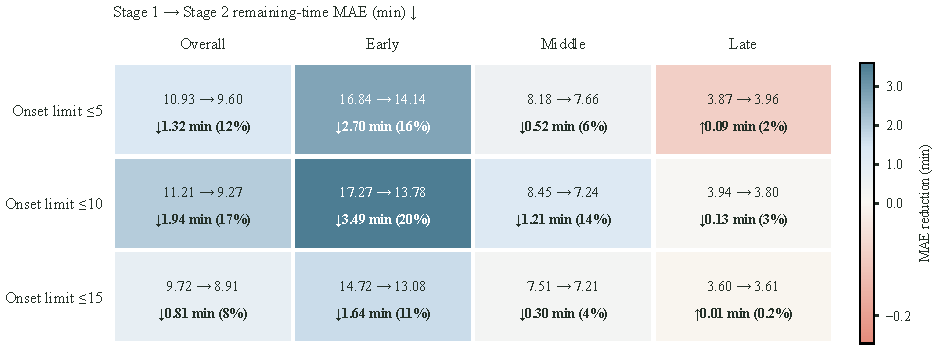
\includegraphics[width=0.90\textwidth,height=0.66\textheight,keepaspectratio]{figures/fig_remain_dumbbell.pdf}
\caption{Effect of remaining-time fine-tuning across early, middle, and late production phases (blue: MAE decrease; coral: increase).}
\label{fig:remain-finetune}
\end{figure}

\FloatBarrier
\section{Evaluation of the proposed components}

The component studies isolate heterogeneous multi-entity representation, process-informed supervision and temporal pattern clustering, and recurrent-pattern-guided delay-aware modelling (Table~\ref{tab:ablation-arms}). Full and all ablation arms share initialization, training budget, curriculum, and validation selection. Remaining-time ablations compare models before head-specific fine-tuning to keep the optimization conditions matched; the fine-tuned full-model results are evaluated in Section~\ref{sec:comparison-remain}. Section~\ref{sec:decoder-training} examines the supporting decoder and training components.

\begin{table}[!htbp]
\centering
\caption{Ablation arms. Every comparison, including the Full reference, begins from identical parameter values and uses the same 50-epoch budget, Onset limit~$\leq5\rightarrow$Onset limit~$\leq10\rightarrow$Onset limit~$\leq15$ curriculum, and validation-controlled model-selection rule.}
\label{tab:ablation-arms}
\footnotesize
\setlength{\tabcolsep}{3.5pt}
\renewcommand{\arraystretch}{1.08}
\begin{tabularx}{\linewidth}{@{}p{0.20\linewidth}p{0.23\linewidth}Y@{}}
\toprule
Arm & Component & Change relative to Full \\
\midrule
NoGraph & Heterogeneous graph & Self-loop adjacency only; no factory edges  \\
NoGroup & Heterogeneous graph & One linear projection of the 27 channels instead of six semantic groups  \\
NoCross & Heterogeneous graph & Within-type edges only; cross-type semantic attention masked  \\
NoInfo & Heterogeneous graph & Only workstations observed; non-workstation features and five coupling channels zeroed  \\
WorkstationOnly & Heterogeneous graph & NoCross and NoInfo combined  \\
NoCluster & Temporal pattern clustering & Temporal pattern clustering removed  \\
NoPattern & \makecell[l]{Delay-aware modelling} & Recent-patch matching to the temporal-pattern prototype bank disabled  \\
NoSplit & Decoder & One shared event-occurrence head for continuing and new events  \\
NoFarBoost & Training & Far-onset weighting and enhanced false-alarm penalty removed  \\
\bottomrule
\end{tabularx}
\end{table}

\subsection{Heterogeneous multi-entity representation}\label{sec:entity-analysis}

Multi-entity ablations assess the contribution of non-workstation observations and cross-resource relations to advance warning. The ablations restrict non-workstation information, cross-type relations, factory edges, or grouped embedding while retaining the same targets (Tables~\ref{tab:ablation-arms} and~\ref{tab:entity-ablation-new}).

\begin{table}[!htbp]
\centering
\caption{Heterogeneous-graph and multi-entity ablation results. Dur. MAE is union error (min); best and second-best values are bold and underlined.}
\label{tab:entity-ablation-new}
\footnotesize
\setlength{\tabcolsep}{3.5pt}
\renewcommand{\arraystretch}{1.05}
\begin{fittable}
\begin{tabular*}{\linewidth}{@{\extracolsep{\fill}}llrrrrr@{}}
\toprule
Arm & \makecell{Onset\\limit} & F1-score & \makecell{Upcoming\\R} & \makecell{Type\\hmean} & \makecell{State F1\\(1 step)} & Dur.\ MAE \\
\midrule
Full & $\leq5$ & \textbf{80.4\%} & \textbf{54.2\%} & \textbf{50.5\%} & \textbf{88.3\%} & \textbf{4.17} \\
NoGraph &  & 74.6\% & 10.4\% & 38.4\% & \underline{87.3\%} & 5.48 \\
NoGroup &  & \underline{75.3\%} & \underline{33.3\%} & \underline{43.2\%} & 83.5\% & \underline{5.11} \\
NoCross &  & 71.6\% & 22.0\% & 39.6\% & 81.2\% & 5.28 \\
NoInfo &  & 64.4\% & 4.9\% & 0.0\% & 69.9\% & 6.66 \\
WorkstationOnly &  & 65.0\% & 3.3\% & 0.0\% & 70.9\% & 6.51 \\
\midrule
Full & $\leq10$ & \textbf{77.8\%} & \textbf{53.5\%} & \textbf{53.0\%} & \textbf{89.2\%} & \textbf{4.38} \\
NoGraph &  & 64.9\% & 6.5\% & 37.6\% & \underline{84.4\%} & 6.46 \\
NoGroup &  & \underline{65.1\%} & \underline{48.5\%} & \underline{45.2\%} & 82.6\% & \underline{6.05} \\
NoCross &  & 57.1\% & 20.7\% & 37.1\% & 75.9\% & 6.60 \\
NoInfo &  & 54.4\% & 2.1\% & 0.0\% & 68.4\% & 7.57 \\
WorkstationOnly &  & 55.9\% & 1.4\% & 0.0\% & 70.8\% & 7.40 \\
\midrule
Full & $\leq15$ & \textbf{76.8\%} & \textbf{53.7\%} & \textbf{53.6\%} & \textbf{90.0\%} & \textbf{4.43} \\
NoGraph &  & \underline{61.2\%} & 3.7\% & 36.0\% & \underline{86.5\%} & 6.57 \\
NoGroup &  & 60.4\% & \underline{43.2\%} & \underline{46.9\%} & 81.9\% & \underline{6.34} \\
NoCross &  & 51.4\% & 31.1\% & 36.5\% & 76.0\% & 6.77 \\
NoInfo &  & 44.1\% & 21.8\% & 0.0\% & 59.6\% & 7.66 \\
WorkstationOnly &  & 53.4\% & 2.1\% & 0.0\% & 70.6\% & 7.46 \\
\bottomrule
\end{tabular*}
\end{fittable}
\end{table}

At Onset limit~$\leq5$, the full representation improves upcoming recall by 50.9 percentage points over WorkstationOnly and by 49.3 points over NoInfo. Removing cross-resource relations or factory edges also weakens distant-event warning (Figure~\ref{fig:cross-resource-evidence}). These comparisons support both the broader observation scope and its relational organization for recognizing constraints that workstation-centred inputs alone fail to reveal.

\begin{figure}[htbp]
\centering
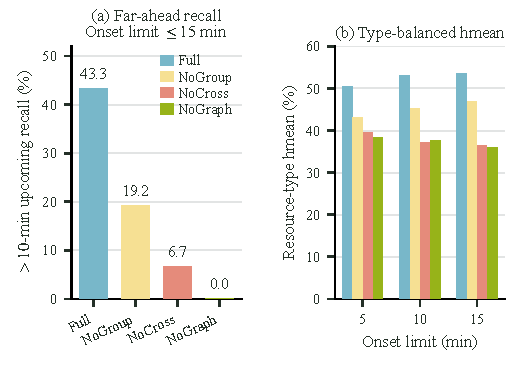
\includegraphics[width=0.82\columnwidth]{figures/fig_cross_resource_evidence.pdf}
\caption{Cross-resource evidence from structural ablations: (a)~far-onset report recall at Onset limit~$\leq15$; (b)~type-hmean F1 across onset limits.}
\label{fig:cross-resource-evidence}
\end{figure}

The complete representation also tracks bottleneck persistence and recovery more closely in Figure~\ref{fig:key-device-entity}. Thus, the heterogeneous graph benefits both advance warning and duration tracking. Resource-level results appear in Appendix~\ref{app:supplementary-results}, with case selection in Appendix~\ref{app:case-details}.

\begin{figure}[!htbp]
\centering
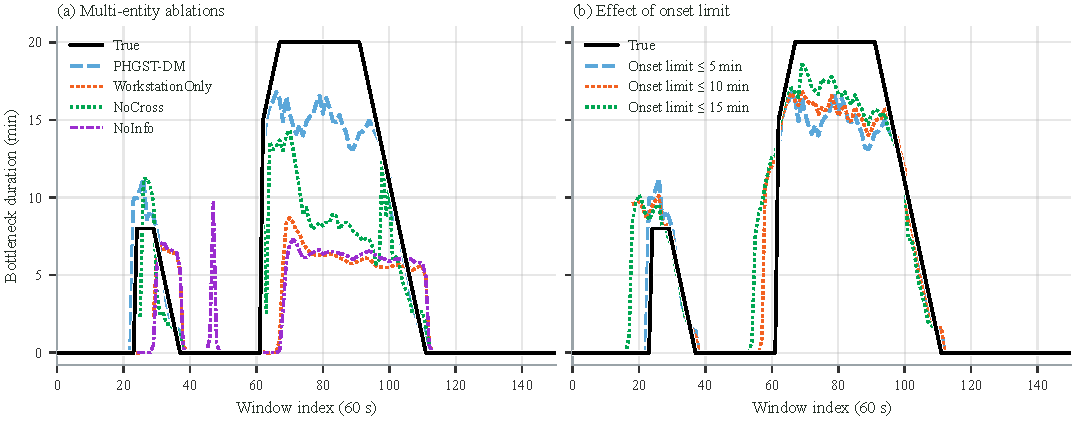
\includegraphics[width=0.96\textwidth,height=0.66\textheight,keepaspectratio]{figures/key_device_entity.pdf}
\caption{Bottleneck-duration traces: panel~(a) compares multi-entity ablations with a 5-min onset limit; panel~(b) compares PHGST-DM with onset limits of 5, 10, and 15~min. The black curve shows the true-duration reference.}
\label{fig:key-device-entity}
\end{figure}

\paragraph*{Cross-resource attention.}\label{sec:attention-protocol}
Figure~\ref{fig:attn-types} examines how the model combines resource information under normal, upcoming, and ongoing bottleneck conditions. Each condition uses 96 episode-stratified test samples, with attention averaged over samples, history steps, heads, and layers. Type-level cells represent mean query-type/attended-type weights. The geographic branch consistently places greater weight on workstations, while the semantic branch exhibits strong workstation--AGV associations and distinct gantry and worker patterns. These associations complement the ablation results by showing how information about production, transport, and workers enters the learned representation. The two branches provide complementary resource views for forecasting constraints whose operational context extends beyond the affected workstation.

\begin{figure}[!htbp]
\centering
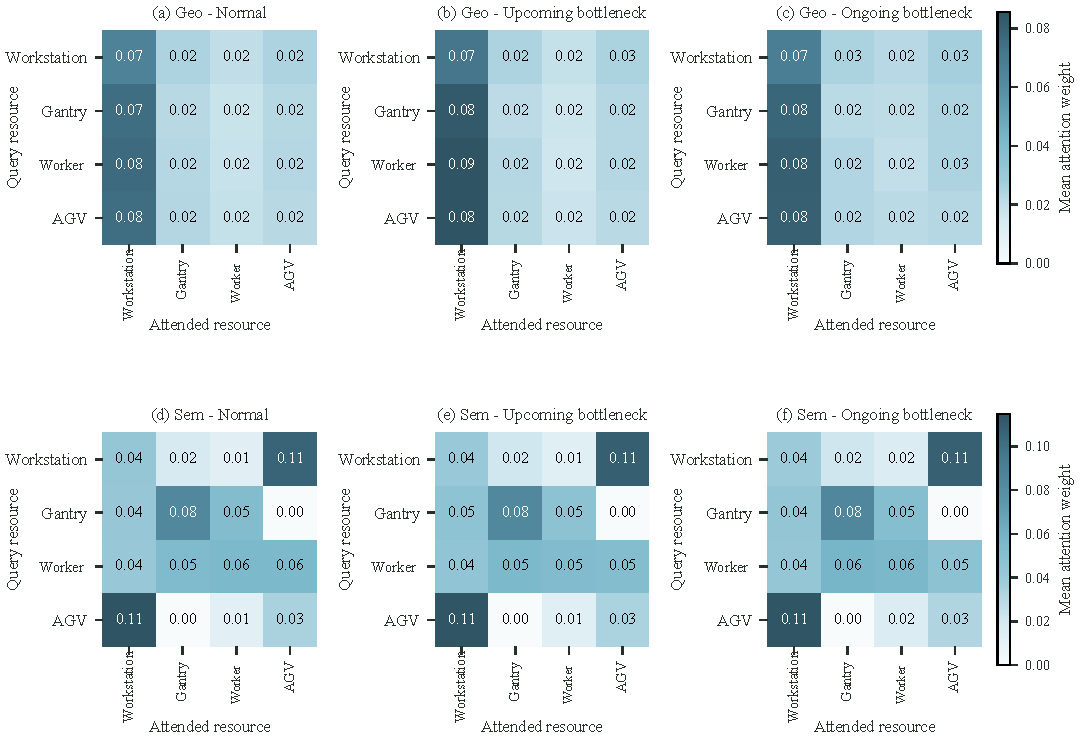
\includegraphics[width=0.92\textwidth,height=0.66\textheight,keepaspectratio]{figures/attention_heatmaps/fig06_entity_type_attention.pdf}
\caption{Type-level attention summary under normal, upcoming, and ongoing conditions (buffers omitted).}
\label{fig:attn-types}
\end{figure}

\subsection{Process-informed supervision and temporal pattern clustering}\label{sec:supervision-analysis}

Three complementary studies address temporal pattern clustering, process-cause supervision, and the production relevance of the constructed event labels.

\paragraph*{(1) Effects of temporal pattern clustering.}
NoCluster tests the predictive value of clustering historical patches into recurrent-pattern prototypes (Table~\ref{tab:group-ablation}); NoPattern separately tests prototype use in Section~\ref{sec:delay-analysis}.

At Onset limit~$\leq15$, temporal pattern clustering improves event F1 by 23.1 percentage points and reduces union duration MAE by 2.22~min relative to NoCluster, a 33.4\% reduction. Gains in upcoming recall and next-window state F1 across the onset limits further show that the pattern bank supports both detection and temporal reconstruction.

\begin{table}[!htbp]
\centering
\caption{Temporal-clustering ablation results. Dur. MAE is union error; Dur. MAE (tp) uses correctly reported events; values are in minutes.}
\label{tab:group-ablation}
\footnotesize
\setlength{\tabcolsep}{3.5pt}
\renewcommand{\arraystretch}{1.08}
\begin{fittable}
\begin{tabular*}{\linewidth}{@{\extracolsep{\fill}}llrrrrr@{}}
\toprule
Arm & \makecell{Onset\\limit} & F1-score & \makecell{Upcoming\\R} & \makecell{State F1\\(1 step)} & Dur.\ MAE & \makecell{Dur. MAE\\(tp)} \\
\midrule
Full & $\leq5$ & \textbf{80.4\%} & \textbf{54.2\%} & \textbf{88.3\%} & \textbf{4.17} & \textbf{1.86} \\
NoCluster & & 73.4\% & 12.5\% & 84.1\% & 5.43 & 2.89 \\
\midrule
Full & $\leq10$ & \textbf{77.8\%} & \textbf{53.5\%} & \textbf{89.2\%} & \textbf{4.38} & \textbf{1.79} \\
NoCluster & & 57.0\% & 34.6\% & 78.9\% & 6.69 & 2.40 \\
\midrule
Full & $\leq15$ & \textbf{76.8\%} & \textbf{53.7\%} & \textbf{90.0\%} & \textbf{4.43} & \textbf{1.72} \\
NoCluster & & 53.7\% & 37.3\% & 81.9\% & 6.65 & 2.30 \\
\bottomrule
\end{tabular*}
\end{fittable}
\end{table}

\paragraph*{(2) Effects of cause supervision.}
The cause-supervision comparison holds labels, data split, onset limit, initialization, seed, and training budget constant (Table~\ref{tab:matched-cause}).

Adding cause supervision improves cause accuracy at the separately selected operating point by 67.0 percentage points and macro recall by 68.2 points, while logged station F1 changes by only 0.2 points.

\begin{table}[!htbp]
\centering
\caption{Matched-budget cause-supervision study at onset limit $\leq5$. Values are percentages.}
\label{tab:matched-cause}
\footnotesize
\setlength{\tabcolsep}{3.5pt}
\renewcommand{\arraystretch}{1.08}
\begin{fittable}
\begin{tabular*}{\linewidth}{@{\extracolsep{\fill}}lrr@{}}
\toprule
Metric & Backbone & +Cause \\
\midrule
Logged station F1 & 73.5\% & 73.3\% \\
Logged cause acc. & 19.5\% & \textbf{89.5\%} \\
Selected cause acc. & 25.2\% & \textbf{92.2\%} \\
Selected cause macro recall & 25.5\% & \textbf{93.7\%} \\
\bottomrule
\end{tabular*}
\end{fittable}
\end{table}

% Evidence: isaac_factory origin/dev_tyx, 8767583f3ed6392cfd8061d4a80de94fcfb9d7a0.
% Source: bottleneck ground-truth validity notes (2026-10-14), checked against label/evaluation code.
% Imported summary values: experiments/data/label_validity_dev_tyx_8767583.json.
\paragraph*{(3) Validation against production sensitivity.}
To assess the production relevance of the event labels, the pilot compares their rankings with order-completion sensitivity under a fixed counterfactual replay protocol. The pilot uses 30 disturbance-free development episodes, separately from predictor training and testing. At a saved factory state, each of seven workstation candidates is accelerated in a separate replay: workstation processing and associated worker-service durations are scaled by $0.8$ (a $1.25\times$ service rate) for 1,200 model steps. Baseline and intervention branches start from the same simulator and random-number states and run to order completion. The reduction in completion time measures production sensitivity. Label methods rank candidates using the preceding three fully observed windows. NDCG@3 measures ranking quality; Positive Recall@$k$ measures top-$k$ coverage; Weighted Recall@3 weights coverage by positive sensitivity; and Coverage@3$_{0.9}$ concerns resources within 90\% of the maximum sensitivity. This fixed acceleration experiment assesses label relevance, not a forecast-guided intervention policy.

\begin{figure}[htbp]
\centering
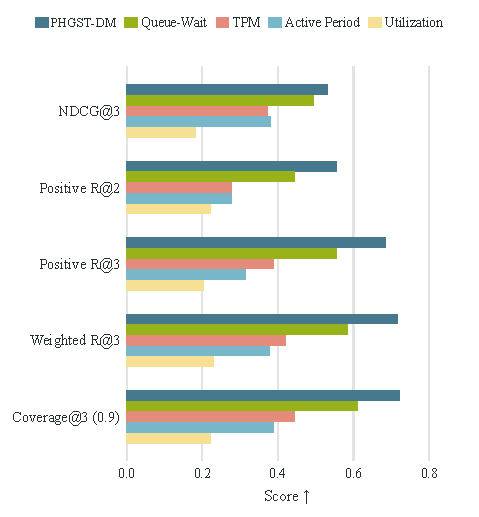
\includegraphics[width=0.76\linewidth,height=0.49\textheight,keepaspectratio]{figures/fig_label_oracle_bars.pdf}
\caption{Counterfactual sensitivity alignment in the exploratory pilot ($\uparrow$: higher is better).}
\label{fig:label-oracle-pilot}
\end{figure}

The process-informed labelling method used by PHGST-DM obtains the highest point estimates on all retained alignment metrics (Figure~\ref{fig:label-oracle-pilot}). Compared with Queue-Wait, NDCG@3 increases by 0.036, Coverage@3$_{0.9}$ improves by 11.1 percentage points, and weighted Recall@3 improves by 13.1 percentage points. Detailed point estimates, reported 95\% confidence intervals for the labelling method, and stage-resolved results are provided in Appendix~\ref{app:supplementary-results}. These exploratory results suggest that combining process evidence helps identify and prioritize resources whose acceleration reduces order-completion time.
\FloatBarrier

\subsection{Delay-aware modelling}\label{sec:delay-analysis}

NoPattern disables recent-patch matching to the fixed prototype bank while retaining the graph and attention branches (Table~\ref{tab:delay-ablation-new}). It isolates historical pattern conditioning from the availability of heterogeneous observations.

At Onset limit~$\leq15$, prototype matching raises strict recall for events more than 10~min ahead by 27.0 percentage points relative to NoPattern, more than doubling distant-event coverage. Improvements in event identification and auxiliary outputs further show that recurrent-pattern conditioning adds forecasting value beyond the heterogeneous graph alone.

This distant-warning benefit supports using earlier resource patterns to anticipate constraints that emerge later, addressing the difficulty of predicting delayed cross-resource effects. Further results appear in Appendix~\ref{app:supplementary-results}.

\begin{table}[!htbp]
\centering
\caption{Temporal-pattern matching ablation in delay-aware modelling. Values compare stage-1 models; onset-distance recall uses strict report matching.}
\label{tab:delay-ablation-new}
\footnotesize
\setlength{\tabcolsep}{2.6pt}
\renewcommand{\arraystretch}{1.08}
\begin{fittable}
\begin{tabular*}{\linewidth}{@{\extracolsep{\fill}}llrrrrrrr@{}}
\toprule
Arm & \makecell{Onset\\limit} & F1-score & \makecell{Upcoming\\R} & $R_{\mathrm{up,rep}}^{6\text{--}10}$ & $R_{\mathrm{up,rep}}^{>10}$ & Queue R & \makecell{Cause\\Macro R} & \makecell{Remain\\MAE} \\
\midrule
Full (stage 1) & $\leq5$ & \textbf{80.4\%} & \textbf{54.2\%} & --- & --- & \textbf{98.4\%} & \textbf{96.7\%} & \textbf{10.93} \\
NoPattern & & 74.5\% & 16.7\% & --- & --- & 14.5\% & 73.4\% & 18.62 \\
\midrule
Full (stage 1) & $\leq10$ & \textbf{77.8\%} & \textbf{53.5\%} & \textbf{46.6\%} & --- & \textbf{98.4\%} & \textbf{96.5\%} & \textbf{11.21} \\
NoPattern & & 58.8\% & 27.8\% & 14.9\% & --- & 47.6\% & 80.5\% & 13.35 \\
\midrule
Full (stage 1) & $\leq15$ & \textbf{76.8\%} & \textbf{53.7\%} & \textbf{52.2\%} & \textbf{43.3\%} & \textbf{98.4\%} & \textbf{97.8\%} & \textbf{9.72} \\
NoPattern & & 60.1\% & 42.7\% & 39.6\% & 16.3\% & 57.3\% & 85.0\% & 11.06 \\
\bottomrule
\end{tabular*}
\end{fittable}
\end{table}

\paragraph*{Historical attention and onset-limit comparisons.}
The descriptive attention maps show that the model draws on multiple historical regions and reweights resource associations across layers and onset limits. The full maps and their interpretation are retained in Appendix~\ref{app:attention-analysis}. These weights describe learned associations and are not evidence of causal effects.

\subsection{Supporting decoder components}\label{sec:decoder-training}

Two decoder-related ablations examine split event heads and far-onset enhancement under the common training and selection protocol (Table~\ref{tab:decoder-ablation}). NoSplit examines the distinction between continuing and newly emerging events; NoFarBoost examines weighting for distant onsets. Each retains its validation-selected operating point.

\begin{table}[!htbp]
\centering
\caption{Split event-head and far-onset ablation results. Thr is the validation-selected threshold; Dur. MAE is union duration error (min).}
\label{tab:decoder-ablation}
\footnotesize
\setlength{\tabcolsep}{3.5pt}
\renewcommand{\arraystretch}{1.08}
\begin{fittable}
\begin{tabular*}{\linewidth}{@{\extracolsep{\fill}}llrrrrrr@{}}
\toprule
Arm & \makecell{Onset\\limit} & Thr & F1-score & \makecell{Upcoming\\R} & $R_{\mathrm{up,rep}}^{>10}$ & \makecell{Ongoing\\R} & Dur.\ MAE \\
\midrule
Full & $\leq5$ & 94.0\% & 80.4\% & 54.2\% & --- & \textbf{93.7\%} & 4.17 \\
NoFarBoost & & 90.0\% & \textbf{81.9\%} & \textbf{54.5\%} & --- & 92.3\% & \textbf{4.03} \\
NoSplit & & 94.0\% & 72.7\% & 19.0\% & --- & 93.5\% & 5.56 \\
\midrule
Full & $\leq10$ & 94.0\% & \textbf{77.8\%} & 53.5\% & --- & 93.9\% & \textbf{4.38} \\
NoFarBoost & & 88.0\% & 75.2\% & \textbf{56.0\%} & --- & 92.3\% & 4.66 \\
NoSplit & & 94.0\% & 58.0\% & 24.7\% & --- & \textbf{94.7\%} & 6.63 \\
\midrule
Full & $\leq15$ & 94.0\% & \textbf{76.8\%} & \textbf{53.7\%} & \textbf{43.3\%} & 93.0\% & \textbf{4.43} \\
NoFarBoost & & 94.0\% & 74.1\% & 48.9\% & 24.0\% & 92.5\% & 4.87 \\
NoSplit & & 94.0\% & 58.6\% & 35.3\% & 12.5\% & \textbf{95.1\%} & 6.36 \\
\bottomrule
\end{tabular*}
\end{fittable}
\end{table}

At Onset limit~$\leq5$, split event heads improve upcoming recall by 35.2 percentage points over NoSplit while retaining high ongoing recall. At Onset limit~$\leq15$, far-onset enhancement raises strict recall beyond 10~min by 19.3 points over NoFarBoost. These gains connect the decoder designs to recognizing newly emerging and more distant events.

Figure~\ref{fig:key-device-struct-graph} shows closer duration tracking by the complete model, with stronger underestimation or post-event spikes in the ablations. Together, the comparisons support decoding that distinguishes current persistence from future onset; weighting benefits remain range-dependent, with NoFarBoost performing better at Onset limit~$\leq5$.

\begin{figure}[!htbp]
\centering
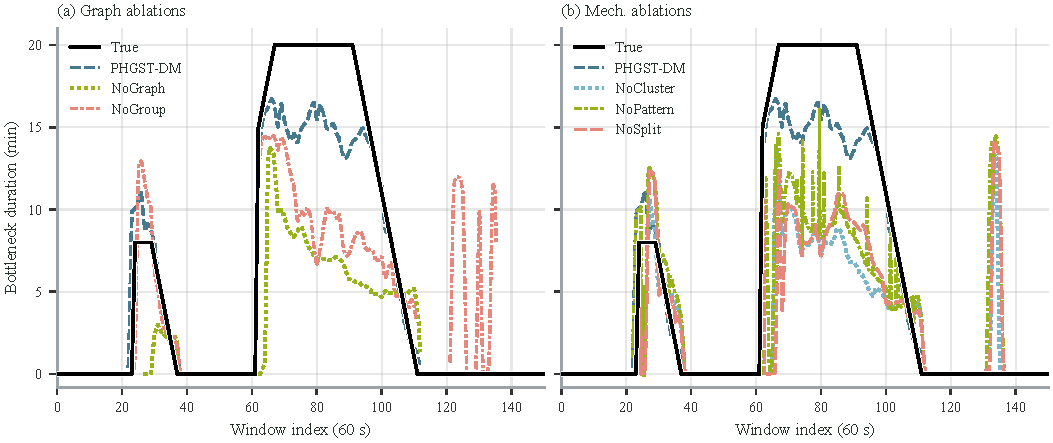
\includegraphics[width=0.96\textwidth,height=0.66\textheight,keepaspectratio]{figures/key_device_struct_pair.pdf}
\caption{Ablation traces (Onset limit~$\leq5$): (a)~graph arms; (b)~process-rule/context, delay-aware modelling, and decoder arms.}
\label{fig:key-device-struct-graph}
\end{figure}

\FloatBarrier
\section{Case study}\label{sec:case-study}

Moving from aggregate results to individual workstation trajectories, the case study assesses predictions of bottleneck onset, duration, and next-window occupancy. The selected episode contains an approximately 8-min bottleneck and a 49-min bottleneck. The prediction horizon is 30~min; the plotted true-duration reference is truncated at 20~min for readability (Figure~\ref{fig:key-device-baselines}). The case is selected by first retaining devices with at least the median event count, then choosing the device with the most events in a single episode, with PHGST-DM one-step F1 breaking ties. Its episode is selected by the number and length of bottleneck segments.

PHGST-DM warns approximately 1~min before the short event, maintains coverage through both intervals, and follows the predicted-duration decline towards recovery. Relative to the baselines, its trajectory contains fewer coverage gaps and follows the sustained constraint more closely (Figure~\ref{fig:key-device-baselines}). Successive forecasts therefore describe bottleneck development through onset, persistence, and recovery.

The workstation state map shows coverage across resources in the same episode (Figure~\ref{fig:all-devices-main}). Full covers the positive cells of both the cutting and second welding workstations, improving episode State F1 by 4.0 percentage points over the strongest ablated configuration, NoGraph. NoInfo and NoCluster miss the welding interval, while NoGraph fragments it. The full model therefore preserves a more complete view of simultaneous workstation constraints within the episode.

% Allow the final experimental figures and Discussion to flow across columns.
\begin{figure}[!htbp]
\centering
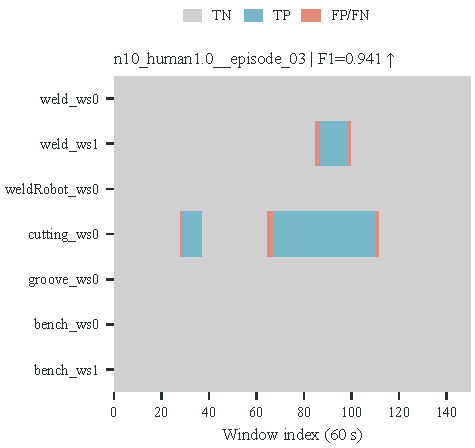
\includegraphics[width=0.82\columnwidth,height=0.66\textheight,keepaspectratio]{figures/all_devices_state_main.pdf}
\caption{Next-window state map for seven workstation targets (grey: TN; light blue: TP; coral: FP/FN). TN, TP, FP, and FN denote true negatives, true positives, false positives, and false negatives, respectively.}
\label{fig:all-devices-main}

\end{figure}



\paragraph*{Resource-level coverage.}
Figure~\ref{fig:per-device} examines whether the joint predictor covers workstations, gantries, and AGVs on the full Onset limit~$\leq5$ test split. Reporting event F1 alongside union duration error separates recognition of an affected resource from reconstruction of its bottleneck interval. The results extend the coverage assessment across resource families and make device-level variation visible instead of hiding it within a single aggregate score.

\begin{center}
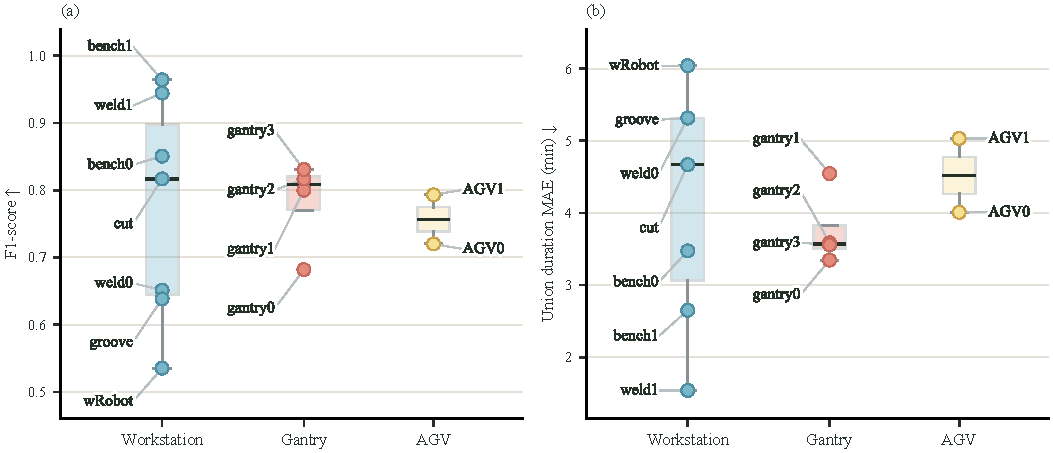
\includegraphics[width=0.95\linewidth,height=0.66\textheight,keepaspectratio]{figures/fig_per_device_box.pdf}
\captionsetup{hypcap=false}
\captionof{figure}{Per-device F1-score and union duration MAE for PHGST-DM at Onset limit~$\leq5$, grouped by resource type: workstation, gantry, and AGV.}
\label{fig:per-device}
\end{center}



